
Este capítulo descreve a abordagem metodológica adotada para o desenvolvimento do interpretador dinâmico proposto, detalhando a arquitetura geral do sistema, as decisões de projeto que sustentam cada fase do compilador implementado e os mecanismos de integração com a plataforma web. A condução do trabalho seguiu as etapas previstas no cronograma do projeto, contemplando, nesta primeira fase do Trabalho de Conclusão de Curso, a revisão bibliográfica, a especificação do escopo da linguagem e de seus elementos configuráveis, a modelagem da arquitetura do interpretador, a implementação das análises léxica e sintática, a geração e a execução do código intermediário e a integração entre o núcleo do compilador e o ambiente web.

A construção do sistema foi conduzida de forma incremental e iterativa, orientada pelas práticas técnicas do \textit{Extreme Programming} discutidas na Seção~\ref{subsec:xp}. Convém explicitar de que modo essas práticas foram efetivamente instanciadas em uma equipe de dois integrantes, uma vez que o método foi adotado de forma parcial e deliberada. Não se estabeleceram ciclos de duração fixa: o trabalho partiu de um conjunto mínimo de requisitos e avançou por acréscimos funcionais, e sempre que uma melhoria não prevista se mostrava pertinente durante a implementação, ela era incorporada naquele momento, em vez de ser postergada para um planejamento posterior. Essa incorporação contínua da mudança, e não a cadência fixa de entregas, é o traço do método que efetivamente governou o projeto \cite{beck2004,wildt2015}.

Quanto à divisão de trabalho, não houve especialização de papéis: ambos os autores atuaram no levantamento de requisitos, no projeto, na implementação, no teste e na revisão, em regime de propriedade coletiva do código, no qual qualquer integrante alterava qualquer parte do sistema, com revisão mútua antes da incorporação ao ramo principal \cite{wildt2015}. As demais práticas foram adotadas nos termos descritos ao longo deste capítulo: o desenvolvimento guiado por testes, detalhado na Seção~\ref{sec:metodologia-testes}; a integração contínua, acionada a cada mudança submetida ao repositório; o \textit{design} simples e a refatoração contínua, que orientaram a organização descrita na Seção~\ref{sec:modelagem-arquitetura}.

O restante deste capítulo está organizado da seguinte maneira. A Seção~\ref{sec:modelagem-arquitetura} descreve a modelagem da arquitetura do projeto; a Seção~\ref{sec:especificacao-linguagem} especifica a linguagem e seus elementos configuráveis; a Seção~\ref{sec:metodologia-interpretador} detalha o núcleo do interpretador, fase a fase; a Seção~\ref{sec:integracao-plataforma} trata da integração entre o núcleo e a plataforma web; e a Seção~\ref{sec:metodologia-testes} expõe a estratégia de testes automatizados.

No ciclo de desenvolvimento guiado por testes adotado, a escrita do teste precede a implementação da funcionalidade: primeiro se especifica o comportamento esperado em um teste que falha, depois se implementa o código necessário para fazê-lo passar e, por fim, se refatora preservando a aprovação da suíte. A integração de uma etapa à seguinte é uma verificação adicional, não o que caracteriza o TDD, conforme a prática consolidada por \citeonline{aniche2012} e \citeonline{martin_coder}. Essa abordagem permitiu a verificação contínua de regressões durante a evolução das configurações da linguagem e a manutenção da estabilidade das fases de análise mesmo diante das frequentes mudanças impostas pela natureza dinâmica da linguagem proposta.

\section{Modelagem da Arquitetura do Projeto}
\label{sec:modelagem-arquitetura}

O sistema está organizado em três unidades de implementação no mesmo repositório: \texttt{packages/compiler}, que contém o núcleo de tradução e execução em TypeScript; \texttt{packages/ide}, que contém a aplicação Next.js e a interface React; e \texttt{backend}, que contém a API de persistência em Python, com FastAPI, SQLAlchemy assíncrono e PostgreSQL. A distinção entre regras de tradução, apresentação e persistência segue o princípio de separação de responsabilidades discutido por \citeonline{martin_clean}. O pacote do núcleo é consumido pela IDE como dependência local e pode ser exercitado diretamente pelos testes, sem depender de uma conexão com o banco de dados.

Cabe explicitar quais padrões de projeto sustentam essa organização. O reconhecimento léxico emprega o padrão \textit{Factory Method}: a classe \texttt{LexerScannerFactory} examina o caractere corrente e devolve o analisador especializado capaz de tratá-lo (\textit{string}, número, comentário, identificador, terminador de instrução ou símbolo), sem que o \texttt{Lexer} precise conhecer as classes concretas. Esses analisadores, por sua vez, materializam o padrão \textit{Strategy}: todos derivam da classe abstrata \texttt{LexerScanner} e implementam a mesma operação \texttt{run}, o que permite acrescentar novas categorias de \textit{token} sem alterar o laço principal da varredura. Já a travessia da sequência de \textit{tokens} pelo analisador sintático segue o padrão \textit{Iterator}, encapsulado na classe \texttt{TokenIterator}, que oferece as operações de avanço, inspeção antecipada e consumo condicional sem expor a estrutura interna da coleção \cite{martin_clean}.

A Figura~\ref{fig:arquitetura-geral-interpretador} distingue os locais de execução. No navegador, os \textit{hooks} \texttt{useLexerAnalyse} e \texttt{useIntermediatorCode} instanciam diretamente o \texttt{Lexer} e o \texttt{TokenIterator}. O primeiro produz os \textit{tokens}; o segundo coordena análise sintática, verificações semânticas e emissão de instruções de três endereços. O componente de terminal instancia o \texttt{Interpreter}, conectando suas funções de entrada e saída à interface. A depuração também reutiliza o núcleo no navegador, por meio de \texttt{useDebugSession}.

\begin{figure}[p]
    \centering
    \caption{Arquitetura e locais de execução do núcleo na plataforma.}
    \label{fig:arquitetura-geral-interpretador}
    % Fonte: hooks da IDE, terminal/body.tsx e pages/api/submissions/validate.ts.
\begin{tikzpicture}[
  box/.style={draw, rounded corners, align=center, text width=11.7cm, inner sep=8pt, font=\small},
  flow/.style={-{Latex},thick},
  note/.style={font=\footnotesize,align=center,fill=white,inner sep=3pt}
]
\node[box,fill=gray!8] (browser) at (0,0) {
  \textbf{Navegador: IDE e núcleo TypeScript}\\[4pt]
  Editor + configuração da linguagem\\
  $\downarrow$\\
  \texttt{Lexer} $\rightarrow$ \textit{tokens} $\rightarrow$ \texttt{TokenIterator} + \texttt{Emitter}\\
  $\downarrow$\\
  Instruções de três endereços $\rightarrow$ \texttt{Interpreter}\\
  $\updownarrow$\\
  Terminal e depuração: entrada, saída e estado da execução
};
\node[box,fill=gray!8] (next) at (0,-5.8) {
  \textbf{Servidor Next.js: avaliação de exercícios}\\[4pt]
  \texttt{POST /api/submissions/validate}\\
  Reutiliza \texttt{Lexer}, \texttt{TokenIterator} e \texttt{Interpreter}\\
  Traduz o programa e executa os casos de teste com entrada simulada
};
\node[box,fill=gray!8] (api) at (0,-9.4) {
  \textbf{Serviço FastAPI + SQLAlchemy}\\[4pt]
  Autenticação; usuários; organizações; linguagens; turmas;\\
  exercícios; listas; submissões
};
\node[box,text width=6cm,fill=gray!8] (db) at (0,-12.1) {
  \textbf{PostgreSQL}\\Persistência das onze tabelas de domínio
};
\draw[flow] (browser.south) -- node[note] {HTTP: código, configuração e identificação do exercício\\Resposta: vereditos dos casos de teste} (next.north);
\draw[flow] (next.south) -- node[note] {HTTP: consulta de casos de teste e registro da submissão} (api.north);
\draw[flow] (api.south) -- node[note] {SQL} (db.north);
\draw[flow] (browser.west) -- ++(-0.8,0) |- (api.west);
\node[note,rotate=90] at (-7.1,-4.2) {HTTP: gestão de recursos};
\end{tikzpicture}

    \legend{Fonte: elaborado pelo autor a partir do código-fonte do projeto.}
\end{figure}

O servidor Next.js reutiliza as mesmas classes na rota \texttt{POST /api/submissions/}\allowbreak\texttt{validate}, destinada à avaliação automática de exercícios. A rota traduz o código recebido, consulta os casos de teste no serviço FastAPI e executa as instruções com entradas simuladas, comparando a saída com o resultado esperado. Os fluxos interativos de análise e de execução da IDE não dependem dessa rota: utilizam o pacote diretamente no navegador. A API FastAPI cuida de autenticação, linguagens, turmas, exercícios e submissões; ela não implementa as fases de tradução do código do estudante.

\subsection{Modelagem do Banco de Dados}
\label{subsec:modelagem-banco}

A persistência utiliza PostgreSQL e um esquema relacional mapeado pelas classes de \texttt{backend/app/models}. A Figura~\ref{fig:esquema-banco} apresenta as onze tabelas de domínio e suas referências. O Apêndice~\ref{ap:dicionario-dados} completa a figura com os 81 atributos, seus tipos, nulabilidade, chaves, restrições e índices extraídos dos metadados SQLAlchemy. Essa documentação descreve a versão do código-fonte examinada em 9 de setembro de 2026; não constitui uma inspeção de um banco de produção.

\begin{landscape}
\begin{figure}[p]
    \centering
    \caption{Tabelas e referências do esquema lógico da plataforma.}
    \label{fig:esquema-banco}
    % Gerado por scripts/gerar-dicionario-dados.py.
\resizebox{0.95\linewidth}{!}{%
\begin{tikzpicture}[entity/.style={draw,rounded corners,fill=white,align=center,text width=3.4cm,minimum height=1.25cm,inner sep=4pt,font=\small},fk/.style={-{Latex},semithick,draw=black!70}]
\node[entity] (n6) at (0,-8) {\texttt{class\_\allowbreak{}exercise\_\allowbreak{}lists}\\7 atributos};
\node[entity] (n3) at (0,-4) {\texttt{class\_\allowbreak{}members}\\3 atributos};
\node[entity] (n4) at (5,-4) {\texttt{classes}\\8 atributos};
\node[entity] (n10) at (10,-12) {\texttt{exercise\_\allowbreak{}list\_\allowbreak{}items}\\4 atributos};
\node[entity] (n9) at (0,-12) {\texttt{exercise\_\allowbreak{}lists}\\8 atributos};
\node[entity] (n5) at (10,-4) {\texttt{exercises}\\9 atributos};
\node[entity] (n2) at (10,0) {\texttt{languages}\\13 atributos};
\node[entity] (n0) at (0,0) {\texttt{organizations}\\3 atributos};
\node[entity] (n7) at (5,-8) {\texttt{submissions}\\11 atributos};
\node[entity] (n8) at (10,-8) {\texttt{test\_\allowbreak{}cases}\\6 atributos};
\node[entity] (n1) at (5,0) {\texttt{users}\\9 atributos};
\begin{scope}[on background layer]
\draw[fk] (n6) -- (n9);
\draw[fk] (n6) -- (n4);
\draw[fk] (n3) -- (n4);
\draw[fk] (n3) -- (n1);
\draw[fk] (n4.north west) -- (n0.south east);
\draw[fk] (n4) -- (n1);
\draw[fk] (n10) -- (n9);
\draw[fk] (n10.east) -- (12.1,-12) -- (12.1,-4) -- (n5.east);
\draw[fk] (n9.east) -- (2.5,-12) -- (2.5,-1.8) -- (n1.south west);
\draw[fk] (n9.south) -- (0,-13.5) -- (12.5,-13.5) -- (12.5,0) -- (n2.east);
\draw[fk] (n5) -- (n1);
\draw[fk] (n5) -- (n2);
\draw[fk] (n2) -- (n1);
\draw[fk] (n2) to[loop above,min distance=18mm] (n2);
\draw[fk] (n7) -- (n5);
\draw[fk] (n7) -- (n9);
\draw[fk] (n7) -- (n4);
\draw[fk] (n7.north east) -- (7.5,-6.5) -- (7.5,-1.8) -- (n1.south east);
\draw[fk] (n8) -- (n5);
\draw[fk] (n1) -- (n0);
\draw[fk] (n1) to[bend left=25] (n2);
\end{scope}
\node[font=\small,align=left,text width=14cm,anchor=north west,inner sep=0pt] at (-1.8,-14.1) {Cada seta parte da tabela que contém a FK e aponta para a tabela referenciada.\\Setas em sentidos opostos entre usuários e linguagens representam propriedade e linguagem ativa. A autorreferência de linguagens registra sua origem por clonagem.};
\end{tikzpicture}}

    \legend{Fonte: elaborado pelo autor a partir dos modelos SQLAlchemy; atributos no Apêndice~\ref{ap:dicionario-dados}.}
\end{figure}
\end{landscape}

O eixo de acesso reúne \texttt{organizations}, \texttt{users}, \texttt{classes} e \texttt{class\_members}. Os usuários compartilham uma tabela e são diferenciados pelo campo \texttt{role}, cujos valores no modelo são \texttt{ADMIN}, \texttt{TEACHER}, \texttt{STUDENT}, \texttt{COMMUNITY} e \texttt{SYSTEM}. O vínculo de um usuário com uma organização é opcional no esquema atual. A turma referencia uma organização e um professor; a associação entre aluno e turma é registrada por uma chave primária composta em \texttt{class\_members}. A existência dessas referências, por si só, não demonstra isolamento de acesso entre organizações, que depende também das regras dos serviços.

A tabela \texttt{languages} registra as linguagens configuradas: proprietário, nome, descrição, configuração em JSONB, dados de imagem, identificador de predefinição e informações de publicação. O campo \texttt{cloned\_from\_id} referencia uma linguagem de origem quando há clonagem, e \texttt{users.active\_language\_id} indica a linguagem ativa do usuário. O par proprietário e nome é único. Esses vínculos permitem documentar a persistência da personalização, ausente no esquema apresentado na qualificação.

O conteúdo pedagógico é distribuído entre \texttt{exercises}, \texttt{test\_cases}, \texttt{exercise\_lists} e \texttt{exercise\_list\_items}. Exercícios e listas possuem política de linguagem \texttt{OPEN} ou \texttt{LOCKED} e uma referência opcional em \texttt{locked\_language\_id}. Uma restrição de verificação exige que essa referência esteja preenchida exatamente quando a política é \texttt{LOCKED}. Os casos de teste pertencem a exercícios e armazenam entrada e saída esperada; os itens de lista associam exercícios a listas, com peso e ordem. A remoção de casos de teste dependentes está configurada no relacionamento do ORM por \texttt{cascade="all, delete-orphan"}, o que deve ser distinguido de uma cláusula SQL \texttt{ON DELETE CASCADE}.

A publicação de uma lista para uma turma é registrada em \texttt{class\_exercise\_lists}, cuja chave primária combina os identificadores da lista e da turma. A tabela armazena prazo, nota total, quantidade mínima de exercícios e instantes de publicação e atualização. Já \texttt{submissions} referencia exercício, lista, turma e estudante e conserva o código e a configuração de linguagem da tentativa nos campos \texttt{code\_snapshot} e \texttt{language\_snapshot}. Seus demais atributos registram o estado da submissão, a pontuação, o comentário do professor e a data de envio. Os valores de estado representam o ciclo de submissão e avaliação; não são, isoladamente, um relatório dos resultados de cada caso de teste.

A separação entre entidades e tabelas associativas segue os conceitos de modelagem relacional discutidos por \citeonline{elmasri2015}. Os instantâneos preservam o contexto de cada tentativa mesmo quando o código ou a linguagem ativa são modificados posteriormente. O relacionamento ORM entre submissão e publicação utiliza os identificadores de lista e turma; o modelo não declara uma chave estrangeira composta de \texttt{submissions} para \texttt{class\_exercise\_lists}. Essa distinção está registrada no dicionário para não atribuir ao banco uma restrição que existe apenas na navegação do ORM. O Alembic gerencia as migrações e mantém a tabela técnica \texttt{alembic\_version}, separada das onze tabelas de domínio.

\subsection{Especificação das Rotas da API}
\label{subsec:rotas-api}

A interface de comunicação entre os clientes e os serviços da plataforma envolve dois modelos distintos de invocação do compilador, combinados com um conjunto de rotas HTTP expostas pelo serviço de persistência. Uma decisão central de arquitetura foi a de que as fases de análise léxica e de geração de código intermediário, cujo resultado é exibido interativamente na IDE, são executadas inteiramente no navegador do usuário, sem qualquer requisição HTTP. Os \textit{hooks} \texttt{useLexerAnalyse} e \texttt{useIntermediatorCode} importam e instanciam diretamente as classes \texttt{Lexer} e \texttt{TokenIterator} do pacote \texttt{compiler}, o que é viável porque esse pacote é escrito em TypeScript puro, sem dependências exclusivas de Node.js para essas operações. Essa abordagem elimina a latência de rede nas interações pedagógicas mais frequentes e mantém o servidor da IDE desonerado das requisições de análise.

A única rota HTTP do pacote \texttt{ide} diretamente relacionada ao compilador é \texttt{POST /api/}\allowbreak\texttt{submissions/}\allowbreak\texttt{validate}. Essa rota, executada no processo do servidor Next.js, recebe o código-fonte e a configuração corrente da linguagem, executa o ciclo completo de análise léxica, geração de código intermediário e interpretação, e avalia o resultado contra os casos de teste do exercício recuperados do serviço de persistência. A rota centraliza a consulta aos casos de teste e o envio da submissão ao serviço de persistência, propagando a credencial recebida nas chamadas HTTP. A implementação inclui um temporizador de cinco segundos por caso, combinado à promessa de execução por \texttt{Promise.race}; esse mecanismo não deve ser confundido com isolamento da execução em um processo separado. Ao término da execução, a rota envia os resultados consolidados ao serviço FastAPI e devolve ao \textit{front-end} a estrutura \texttt{TValidationResult}, contendo o status de cada caso de teste, a pontuação obtida e eventuais avisos de compilação.

As demais rotas HTTP da plataforma pertencem ao serviço de persistência, implementado em Python com o \textit{framework} FastAPI e o ORM SQLAlchemy assíncrono. A documentação completa e interativa dessas rotas é gerada automaticamente pelo próprio \textit{framework}, conforme descrito por \citeonline{fastapi2026}, e está disponível nos endereços \url{https://api.dynamicinterpreter.com.br/docs} (interface Swagger UI) e \url{https://api.dynamicinterpreter.com.br/redoc} (interface ReDoc). Essas rotas organizam-se nos seguintes grupos de recursos:

\begin{itemize}
    \item \textbf{Autenticação} (\texttt{/auth}): gerencia o registro e o \textit{login} de usuários, emitindo tokens JWT utilizados nas demais requisições protegidas;
    \item \textbf{Linguagens} (\texttt{/languages}): gerencia configurações nomeadas, publicação no catálogo e importação de linguagens;
    \item \textbf{Organizações} (\texttt{/organizations}): gerencia as instituições de ensino cadastradas na plataforma, às quais professores e alunos são vinculados;
    \item \textbf{Usuários} (\texttt{/users}): expõe operações de consulta e atualização de perfil, com controle de acesso baseado no atributo \texttt{role};
    \item \textbf{Turmas} (\texttt{/classes}): permite ao professor criar, editar, encerrar e arquivar turmas; a matrícula de estudantes é realizada por meio do código de acesso único da turma, gerenciado pela sub-rota \texttt{/classes/join};
    \item \textbf{Exercícios} (\texttt{/exercises}): centraliza a criação e a manutenção dos enunciados de exercícios, incluindo seus casos de teste, com restrição de escrita ao professor responsável;
    \item \textbf{Listas de exercícios} (\texttt{/exercise-lists}): gerencia a composição e a ordenação dos exercícios em uma lista, com controle de pesos de nota por item;
    \item \textbf{Publicação de listas} (\texttt{/class-exercise-lists}): controla a associação de uma lista a uma turma, registrando prazo, nota total e mínimo de exercícios exigidos;
    \item \textbf{Submissões} (\texttt{/submissions}): armazena e recupera os registros de submissão dos estudantes, incluindo o instantâneo do código, a pontuação e a retroalimentação do professor.
\end{itemize}

Essa organização reflete diretamente a divisão arquitetural do projeto: o compilador opera localmente no navegador para as interações pedagógicas de baixa latência, em uma rota de servidor para a avaliação controlada de submissões, e o serviço FastAPI permanece inteiramente agnóstico em relação ao compilador, concentrando-se exclusivamente na gestão das entidades de domínio pedagógico. A relação completa dos grupos de recursos da API está reproduzida no Apêndice~\ref{ap:api}.

\section{Especificação da Linguagem e de seus Elementos Configuráveis}
\label{sec:especificacao-linguagem}

A linguagem suportada pelo interpretador foi projetada como uma linguagem imperativa didática, com variantes de tipagem configuráveis, suficientemente expressiva para abranger os conteúdos típicos das disciplinas introdutórias de programação, e simultaneamente flexível para que professores e alunos possam customizar suas regras superficiais. O conjunto base de funcionalidades contempla declarações de variáveis com tipagem estática, atribuições, expressões aritméticas, lógicas e relacionais, estruturas condicionais (\texttt{if}/\texttt{else} e \texttt{switch}), estruturas de repetição (\texttt{for} e \texttt{while}), arranjos uni e multidimensionais com modos de alocação fixos e dinâmicos, e operações de entrada e saída padrão (\texttt{print} e \texttt{scan}).

A configuração foi motivada pela investigação de escolhas sintáticas no ensino de programação \cite{stefik2013}. No núcleo implementado, \texttt{LexerConfig} reúne os mapeamentos de palavras-chave, operadores, literais booleanos, delimitadores e terminador, além da opção de indentação. Essas escolhas alteram a forma de reconhecer elementos cuja interpretação interna já está definida. A Tabela~\ref{tab:elementos-configuraveis} apresenta as possibilidades de redefinição lexical e suas restrições.

O tipo \texttt{GrammarConfig}, recebido por \texttt{TokenIterator}, reúne quatro seleções: terminadores obrigatórios ou opcionais no fim da linha; blocos delimitados ou por indentação; modo com declaração explícita de tipo ou modo sem essa declaração; e arranjos fixos ou dinâmicos. Essas opções selecionam alternativas já codificadas no analisador e nos descritores semânticos. A palavra dinâmico no título não equivale especificamente ao modo de tipagem: refere-se ao recebimento dessa configuração para um novo processamento, sem a geração de um analisador arbitrário pelo usuário.

\begin{table}[htbp]
    \centering
    \caption{Elementos da linguagem passíveis de redefinição pelo usuário.}
    \label{tab:elementos-configuraveis}
    \footnotesize
    \setlength{\tabcolsep}{4pt}
    \renewcommand{\arraystretch}{1.25}
    \begin{tabular}{|>{\raggedright\arraybackslash}p{2.5cm}|>{\raggedright\arraybackslash}p{2.6cm}|>{\raggedright\arraybackslash}p{2.9cm}|>{\raggedright\arraybackslash}p{5.2cm}|}
        \hline
        \textbf{Elemento} & \textbf{Forma canônica} & \textbf{Exemplo de personalização} & \textbf{Restrições verificadas} \\
        \hline
        Palavras-chave de tipo & \texttt{int}, \texttt{float}, \texttt{bool}, \texttt{string} & \texttt{inteiro}, \texttt{real}, \texttt{logico}, \texttt{texto} & Devem ter forma de identificador e não colidir entre si nem com os demais elementos configurados \\
        \hline
        Controle de fluxo & \texttt{if}, \texttt{else}, \texttt{for}, \texttt{while}, \texttt{break}, \texttt{continue}, \texttt{return} & \texttt{se}, \texttt{senao}, \texttt{para}, \texttt{enquanto}, \texttt{pare}, \texttt{siga}, \texttt{retorne} & Mesmas restrições das palavras-chave de tipo \\
        \hline
        Entrada e saída & \texttt{print}, \texttt{scan} & \texttt{escreva}, \texttt{leia} & Mesmas restrições das palavras-chave de tipo \\
        \hline
        Operadores lógicos & \texttt{\&\&}, \texttt{||}, \texttt{!} & \texttt{e}, \texttt{ou}, \texttt{nao} & Forma de identificador; sem duplicatas; não podem reusar palavra reservada nem colidir com delimitadores de bloco \\
        \hline
        Operadores relacionais & \texttt{==}, \texttt{!=}, \texttt{>}, \texttt{>=}, \texttt{<}, \texttt{<=} & \texttt{igual}, \texttt{diferente}, \texttt{maior}, \texttt{maiorIgual}, \texttt{menor}, \texttt{menorIgual} & Mesmas restrições dos operadores lógicos \\
        \hline
        Literais booleanos & \texttt{true}, \texttt{false} & \texttt{verdadeiro}, \texttt{falso} & Forma de identificador; sem duplicatas; não podem conflitar com operadores em forma de palavra nem com delimitadores \\
        \hline
        Delimitadores de bloco & \texttt{\{} e \texttt{\}} & \texttt{inicio} e \texttt{fim}, ou indentação & Ambos preenchidos, com forma de identificador, distintos entre si e sem reusar palavra reservada \\
        \hline
        Terminador de instrução & \texttt{;} & \texttt{ponto} ou ausência de terminador & Não pode ser vazio, conter espaços, reusar o ponto e vírgula ou caracteres de operadores fixos, nem colidir com palavras já definidas na linguagem \\
        \hline
    \end{tabular}
    \legend{Fonte: elaborado pelo autor, a partir das funções de validação do módulo \texttt{config.ts} do pacote \texttt{compiler}.}
\end{table}


A validação prévia da configuração é tratada por funções utilitárias dedicadas, como \texttt{validateOperator}\allowbreak\texttt{WordMap}, \texttt{validateBoolean}\allowbreak\texttt{LiteralMap}, \texttt{validateBlock}\allowbreak\texttt{Delimiters} e \texttt{validateStatement}\allowbreak\texttt{TerminatorLexeme}. Cada uma dessas funções verifica restrições léxicas elementares antes do início da análise, impedindo, por exemplo, que palavras-chave personalizadas colidam com identificadores válidos ou que delimitadores de bloco contenham caracteres inválidos. Essa estratégia preventiva atende aos princípios de detecção precoce de erros discutidos por \citeonline{cooper2012}, transformando inconsistências de configuração em mensagens claras antes mesmo da leitura do código-fonte. A Figura \ref{fig:validate-functions} apresenta a implementação das quatro funções de validação.

\begin{figure}[p]
    \centering
    \caption{Funções de validação prévia da configuração léxica da linguagem.}
    \label{fig:validate-functions}
    \begin{subfigure}[t]{0.48\textwidth}
        \centering
        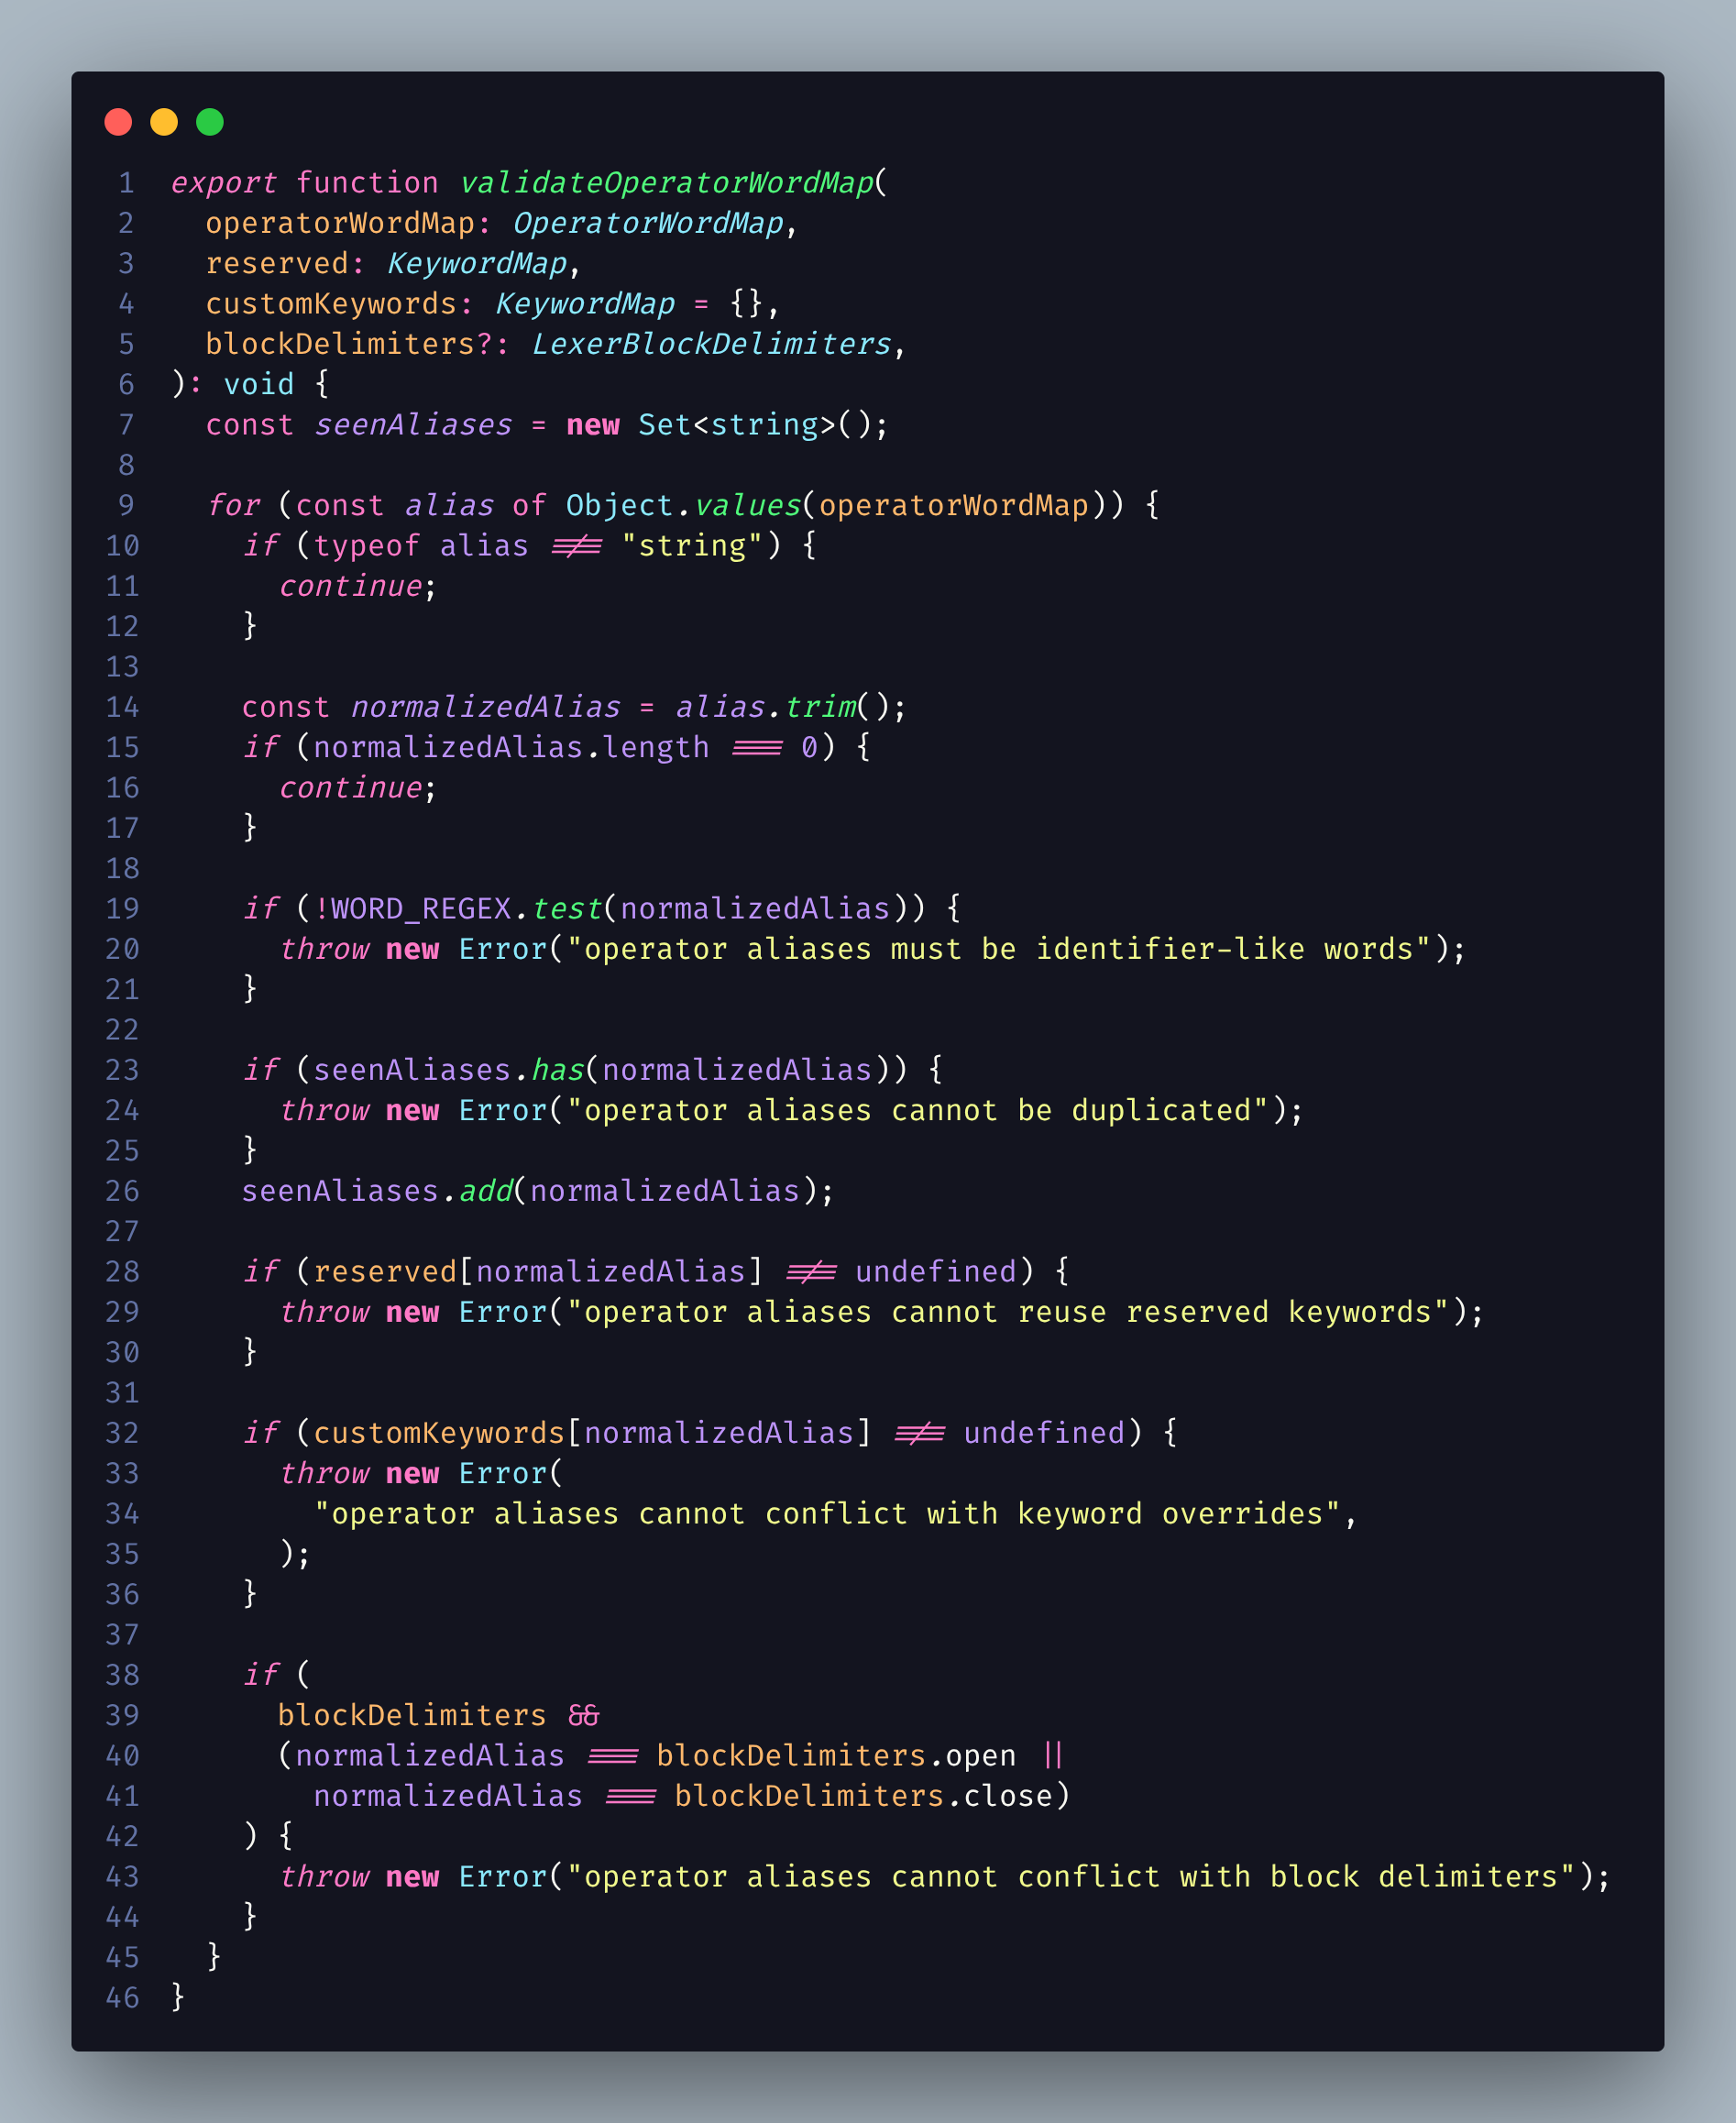
\includegraphics[width=\textwidth,height=0.27\textheight,keepaspectratio]{Figuras/validateOperatorWordMap.png}
        \caption{\texttt{validateOperator}\allowbreak\texttt{WordMap}}
        \label{fig:validate-operator-word-map}
    \end{subfigure}
    \hfill
    \begin{subfigure}[t]{0.48\textwidth}
        \centering
        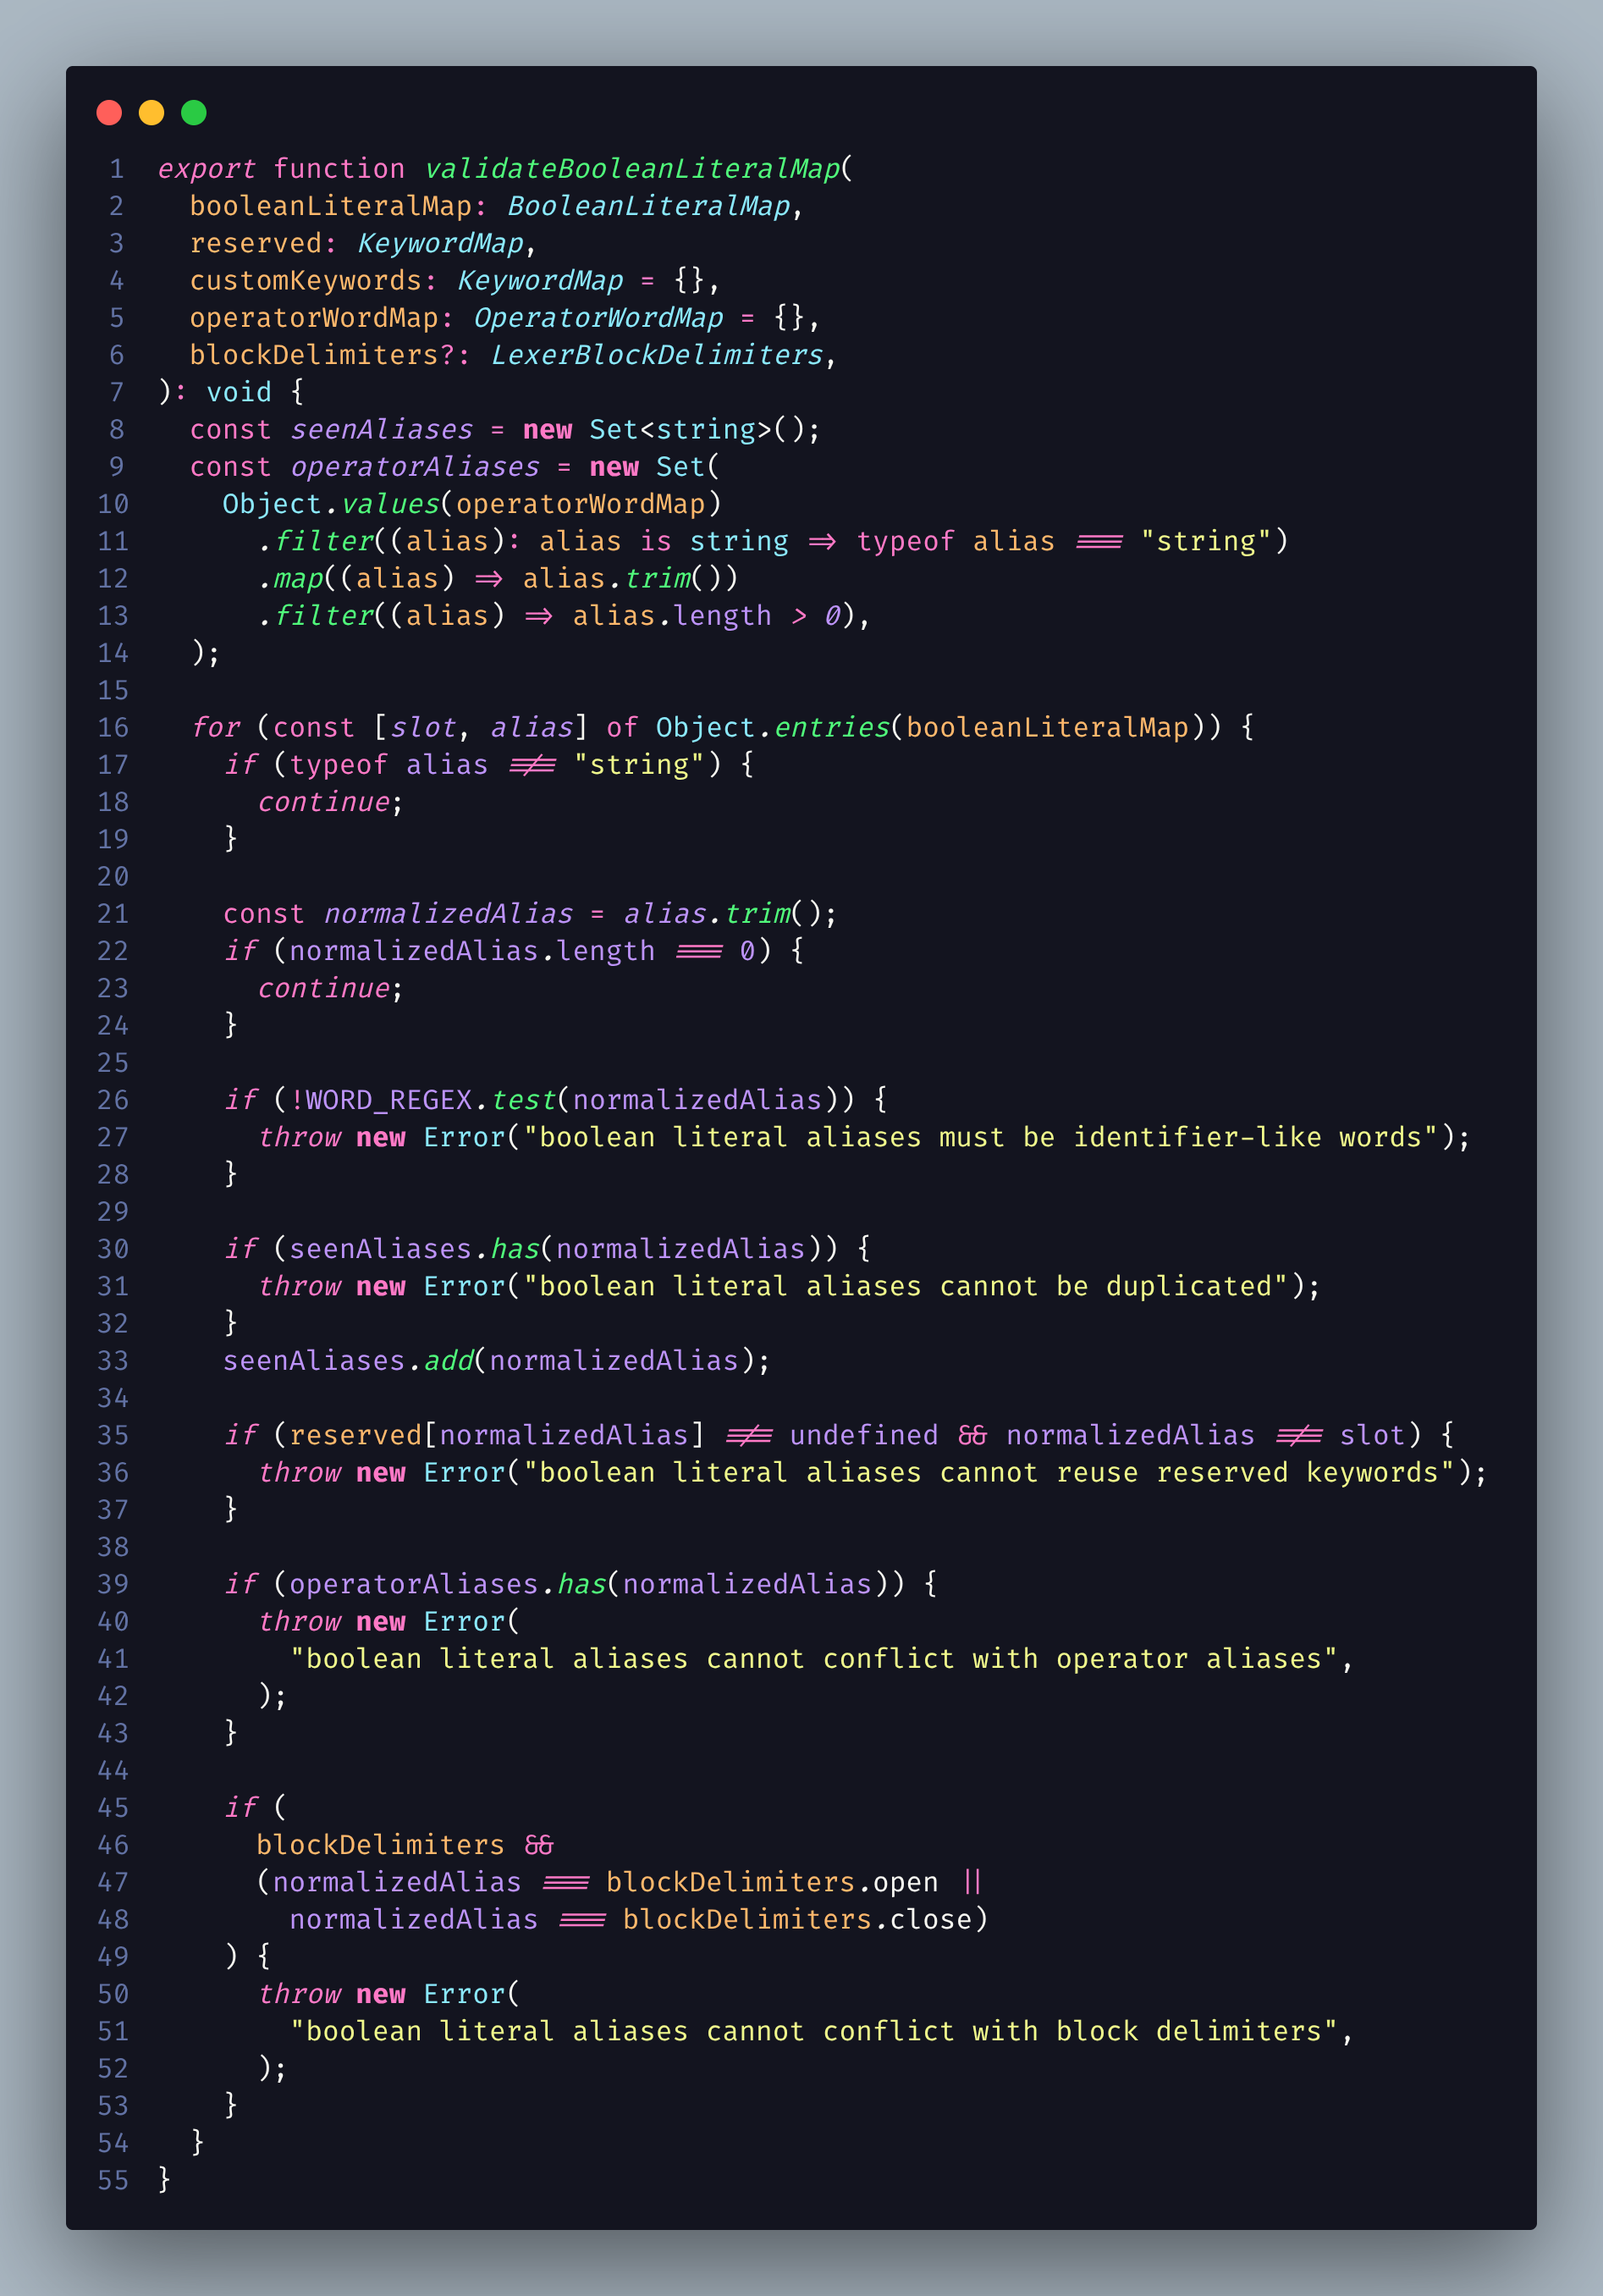
\includegraphics[width=\textwidth,height=0.27\textheight,keepaspectratio]{Figuras/validateBooleanLiteralMap.png}
        \caption{\texttt{validateBoolean}\allowbreak\texttt{LiteralMap}}
        \label{fig:validate-boolean-literal-map}
    \end{subfigure}

    \vspace{0.8em}

    \begin{subfigure}[t]{0.48\textwidth}
        \centering
        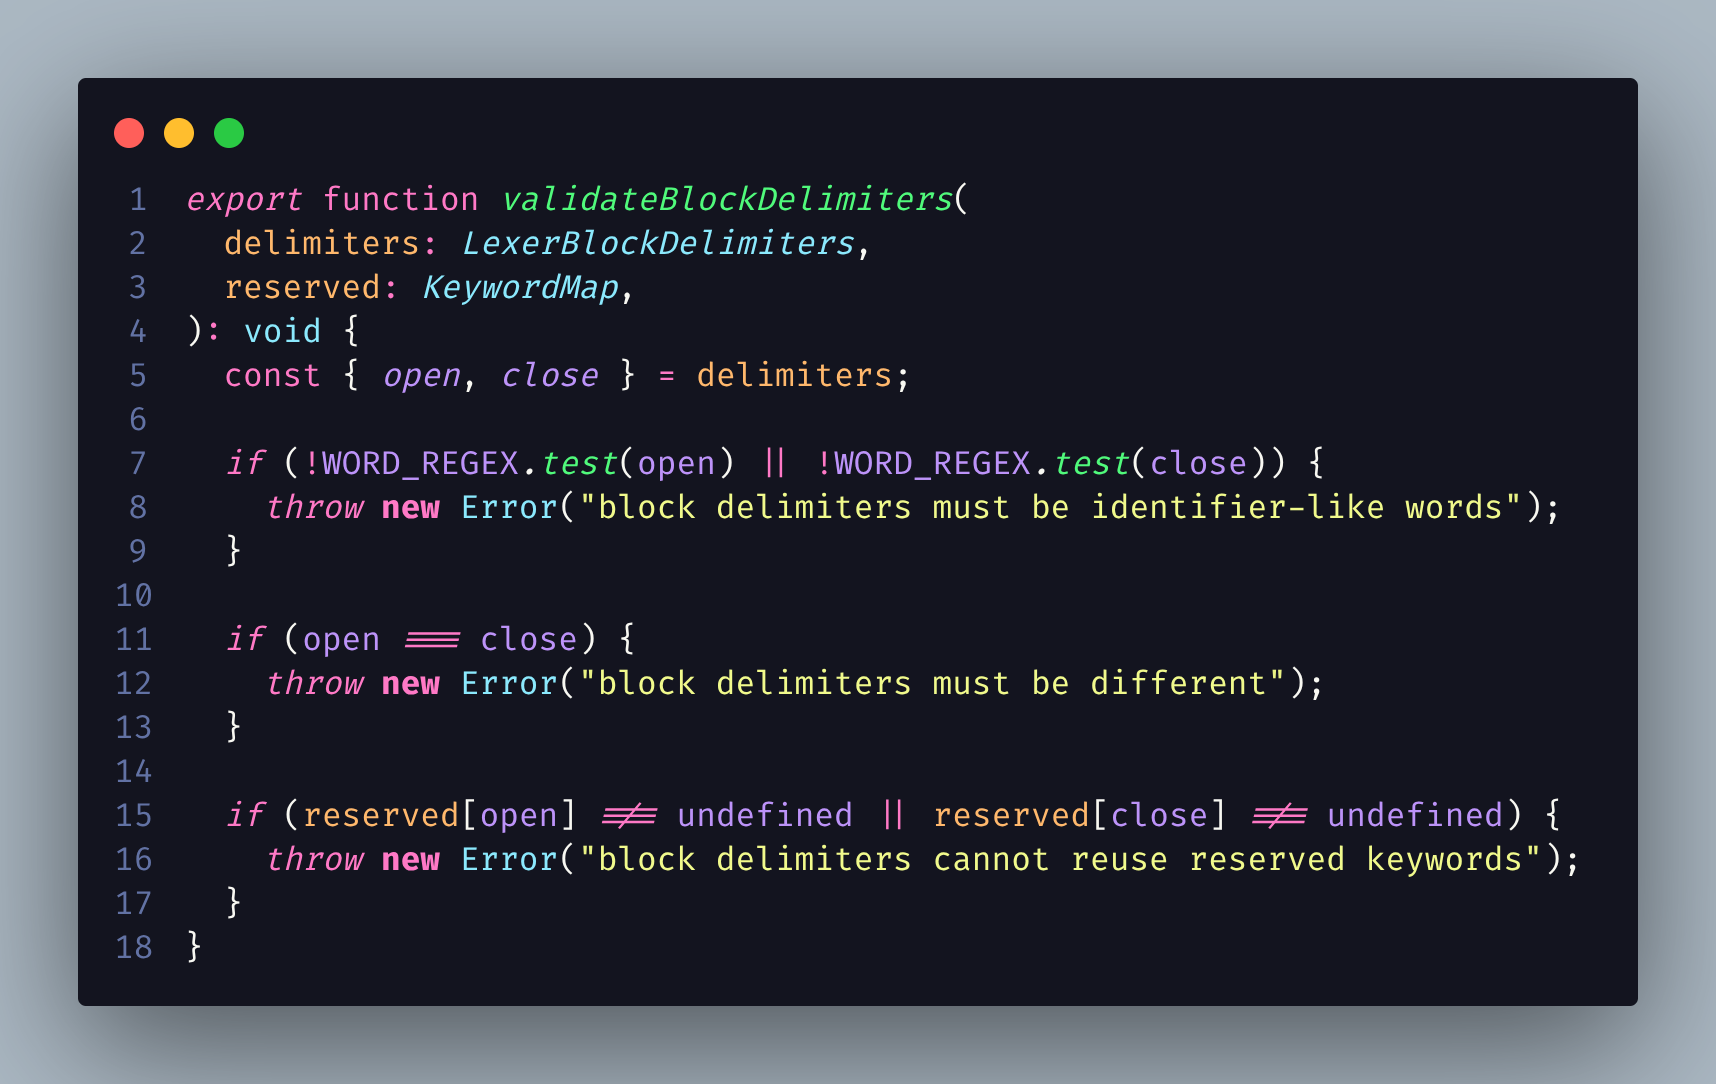
\includegraphics[width=\textwidth,height=0.27\textheight,keepaspectratio]{Figuras/validateBlockDelimiter.png}
        \caption{\texttt{validateBlock}\allowbreak\texttt{Delimiters}}
        \label{fig:validate-block-delimiter}
    \end{subfigure}
    \hfill
    \begin{subfigure}[t]{0.48\textwidth}
        \centering
        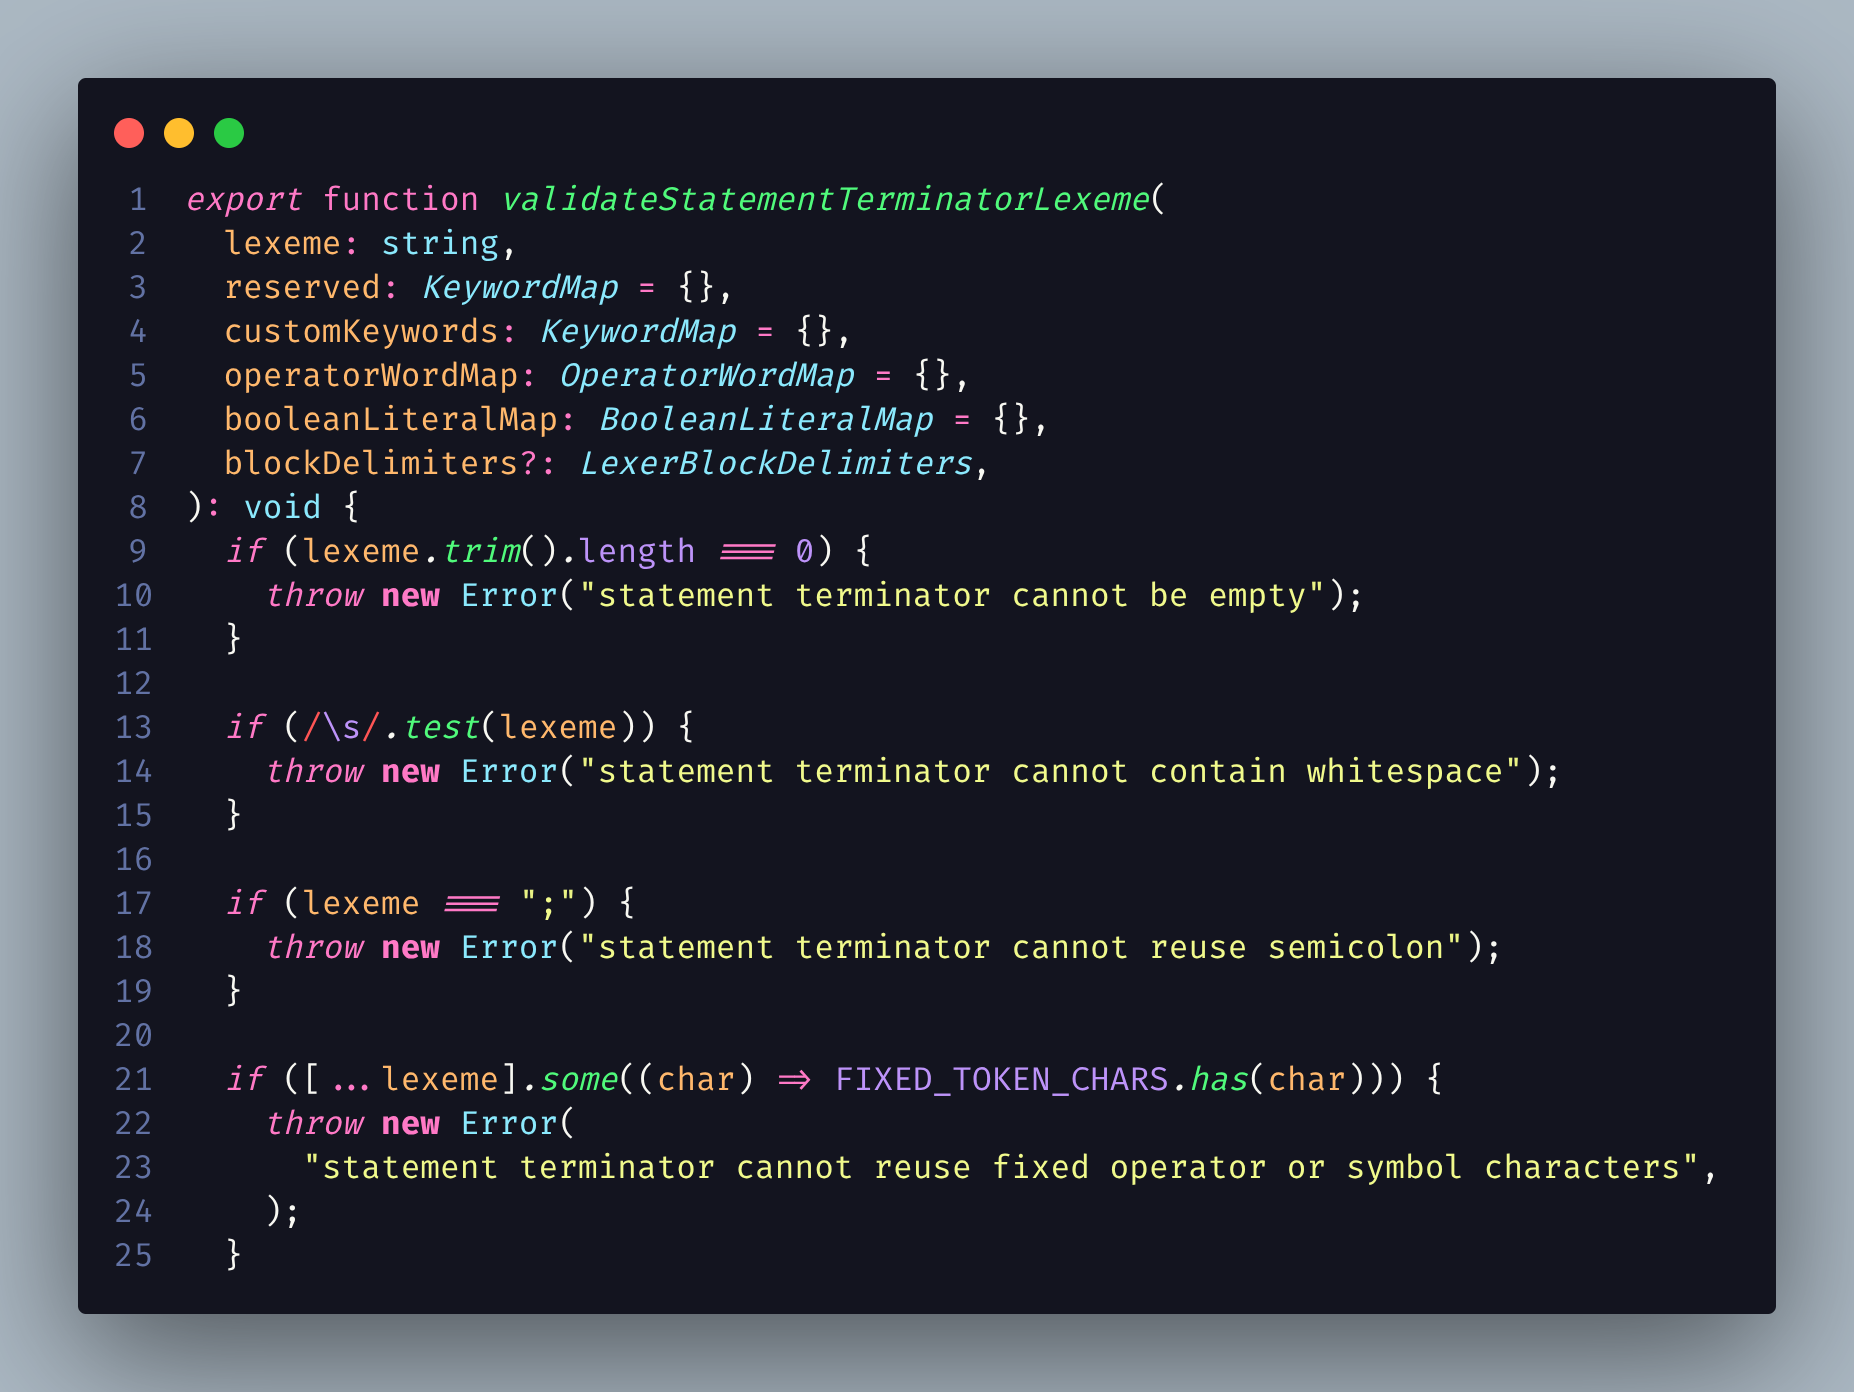
\includegraphics[width=\textwidth,height=0.27\textheight,keepaspectratio]{Figuras/validateStatementTerminatorLexeme.png}
        \caption{\texttt{validateStatement}\allowbreak\texttt{TerminatorLexeme}}
        \label{fig:validate-statement-terminator}
    \end{subfigure}
    \legend{Fonte: elaborado pelo autor.}
\end{figure}

\clearpage
\section{Interpretador}
\label{sec:metodologia-interpretador}

O desenvolvimento do interpretador descrito nesta seção, que abrange as fases de análise léxica, sintática e semântica, a geração de código intermediário e a execução do código, constitui o núcleo comum do projeto e foi conduzido de forma colaborativa pelos dois autores, Victor de Souza Vilela da Silva e Igor Lamoia Queiroz, conforme detalhado no Apêndice~\ref{ap:plano}. O núcleo de tradução foi implementado em TypeScript, reutilizado no servidor Next.js para avaliar exercícios e no navegador para análise, geração de instruções, execução no terminal e depuração, conforme a Figura~\ref{fig:arquitetura-geral-interpretador}. A escolha pela linguagem TypeScript permitiu o uso intensivo do sistema de tipos durante o desenvolvimento, aproximando o processo de implementação dos benefícios de verificação estática descritos por \citeonline{aho1995} e \citeonline{martin_clean_code}, e contribuindo para a robustez das estruturas de dados que atravessam todas as fases do compilador.

\subsection{Análise Léxica}
\label{subsec:analise-lexica}

A análise léxica foi implementada na classe \texttt{Lexer}, que percorre o código-fonte caractere por caractere e produz uma lista ordenada de instâncias da classe \texttt{Token}. Cada \textit{token} carrega quatro atributos essenciais à fase seguinte e à emissão de erros: um identificador numérico (\texttt{type}), associado a uma das categorias léxicas suportadas pela linguagem, o lexema literalmente lido do código-fonte, a linha e a coluna em que o lexema iniciou-se. Essa estrutura está alinhada à distinção teórica entre lexema e \textit{token} discutida por \citeonline{nystrom2021} e foi mantida estável ao longo de todo o desenvolvimento, pois constitui a interface entre o \textit{front-end} e o restante do compilador. A decomposição de uma instrução em sua sequência de \textit{tokens} segue o conceito ilustrado na Figura~\ref{fig:lexemas_nystrom}, apresentada no referencial teórico.

Os \textit{tokens} foram organizados em sete grupos temáticos, a saber: aritméticos, lógicos, relacionais, atribuições, palavras reservadas, símbolos e literais, cada um deles definido em um módulo próprio sob o diretório \texttt{token/constants}. Essa segregação favorece a manutenção da tabela de \textit{tokens} e habilita o uso de estilos visuais distintos por categoria na IDE, alinhados aos campos \texttt{TOKENS\_STYLE} associados a cada grupo. A tabela completa de tipos é exportada também na forma invertida (\texttt{BY\_ID}), o que viabiliza a tradução reversa de identificadores numéricos em descrições legíveis, fundamental para fins de depuração e visualização pedagógica.

A escolha por uma análise léxica determinística orientada por caracteres em vez de geradores automáticos como \textit{Lex} foi motivada pela natureza dinâmica das palavras-chave da linguagem proposta. Como o vocabulário não é fixo em tempo de compilação, autômatos finitos pré-gerados perderiam a flexibilidade exigida pelo projeto. Em substituição, adotou-se o padrão \textit{Factory} no diretório \texttt{lexer/scanners}, no qual a função \texttt{LexerScannerFactory.}\allowbreak\texttt{getInstance()} despacha o caractere corrente para o \textit{scanner} apropriado: \texttt{comment.ts} para comentários de linha e de bloco, \texttt{identifier.ts} para identificadores e palavras-chave, \texttt{number.ts} para literais inteiros e em ponto flutuante, \texttt{string.ts} para literais de cadeia com sequências de escape, e \texttt{symbol-and-}\allowbreak\texttt{operator.ts} para os demais símbolos. Um \textit{scanner} adicional, \texttt{statement-}\allowbreak\texttt{terminator.ts}, é instanciado dinamicamente conforme o terminador de instrução configurado pelo usuário, podendo assumir caracteres distintos do ponto e vírgula tradicional ou mesmo ser desativado. A Tabela~\ref{tab:scanners} sintetiza os analisadores especializados e suas respectivas responsabilidades.

\begin{table}[H]
    \centering
    \caption{Analisadores especializados (\textit{scanners}) despachados pela \texttt{LexerScannerFactory}.}
    \label{tab:scanners}
    \begin{tabular}{|l|p{9.2cm}|}
        \hline
        \textbf{\textit{Scanner}} & \textbf{Responsabilidade} \\
        \hline
        \texttt{comment.ts} & Comentários de linha (\texttt{//}) e de bloco (\texttt{/* */}). \\
        \hline
        \texttt{identifier.ts} & Identificadores e palavras-chave, classificados conforme o vocabulário ativo na configuração corrente. \\
        \hline
        \texttt{number.ts} & Literais inteiros e em ponto flutuante. \\
        \hline
        \texttt{string.ts} & Literais de cadeia, incluindo o tratamento de sequências de escape. \\
        \hline
        \texttt{symbol-and-operator.ts} & Operadores e demais símbolos da linguagem. \\
        \hline
        \texttt{statement-terminator.ts} & Terminador de instrução configurável, instanciado dinamicamente conforme a configuração do usuário. \\
        \hline
    \end{tabular}
    \legend{Fonte: elaborado pelo autor.}
\end{table}

A função \texttt{buildEffective}\allowbreak\texttt{KeywordMap}, alimentada pela configuração de personalização proveniente da IDE, constrói em tempo de execução o mapeamento entre os lexemas das palavras-chave correntes e os identificadores numéricos canônicos dos \textit{tokens}. Dessa forma, ao reconhecer um identificador no código-fonte, o analisador léxico verifica primeiro se o lexema corresponde a alguma palavra-chave ativa naquela configuração, classificando-o como \texttt{reserved} quando aplicável e como identificador comum caso contrário. Esse mecanismo concentra toda a flexibilidade linguística no analisador léxico, mantendo os estágios subsequentes inalterados ainda que o vocabulário superficial mude entre execuções.

A análise léxica também é responsável pelo modo de delimitação de blocos. Quando a IDE indica que o usuário optou por blocos baseados em indentação, em substituição às chaves, o \textit{lexer} emite \textit{tokens} sintéticos de \texttt{indent}, \texttt{dedent} e \texttt{newline} em pontos apropriados, aproveitando o registro contínuo de coluna e o tamanho de tabulação configurado pelo usuário. Esse comportamento foi inspirado nas linguagens estruturadas por indentação e permite que a etapa de análise sintática mantenha uma única gramática base, alternando entre blocos delimitados por chaves ou por indentação a partir do conjunto de \textit{tokens} efetivamente gerado.

\subsection{Análise Sintática}
\label{subsec:analise-sintatica}

A análise sintática foi implementada por meio de um analisador descendente recursivo, materializado no diretório \texttt{grammar/syntax}. A escolha por esta estratégia, em detrimento das famílias \textit{bottom-up} discutidas por \citeonline{aho1995}, decorreu de três fatores: a clareza pedagógica da correspondência direta entre regras de produção e funções TypeScript, a facilidade de emissão de mensagens de erro contextualizadas, e a aderência natural ao requisito de visualização passo a passo do processo de compilação dentro da IDE. Cada não-terminal da gramática foi materializado em um arquivo dedicado, como \texttt{stmt.ts}, \texttt{ifStmt.ts}, \texttt{forStmt.ts}, \texttt{whileStmt.ts}, \texttt{switchStmt.ts}, \texttt{declarationStmt.ts}, \texttt{ioStmt.ts} e \texttt{functionCallExpr.ts}, contendo, em comentários, a derivação formal correspondente.

A navegação sobre a sequência de \textit{tokens} produzida pelo analisador léxico foi encapsulada na classe \texttt{TokenIterator}, que oferece operações de \texttt{peek}, \texttt{next}, \texttt{consume} e \texttt{match}, além de mecanismos de consulta ao modo de bloco e ao modo de tipagem corrente. O isolamento dessas operações em um único componente padroniza a forma como cada produção avança sobre o fluxo de \textit{tokens} e protege o restante do analisador de possíveis erros de manipulação direta, como leituras fora dos limites ou consumos indevidos. Esta organização materializa o princípio do Padrão Iterador discutido por \citeonline{silveira2012}.

A gramática base foi cuidadosamente fatorada à esquerda e mantida livre de recursão à esquerda, conforme as restrições necessárias à análise preditiva discutidas por \citeonline{aho1995}. Para acomodar as variações configuráveis pelo usuário, a função \texttt{consumeStmt}\allowbreak\texttt{Terminator} centraliza a verificação do terminador de instrução, podendo aceitar ponto e vírgula, lexemas alternativos definidos pelo usuário ou mesmo nenhum terminador, conforme a configuração ativa. O mesmo princípio governa o tratamento dos delimitadores de bloco: quando a IDE comunica ao analisador o modo indentado, o reconhecimento de \texttt{left\_brace} e \texttt{right\_brace} é substituído pelo casamento dos \textit{tokens} sintéticos \texttt{indent} e \texttt{dedent} gerados pelo \textit{lexer}, mantendo o restante da gramática inalterado.

\subsection{Análise Semântica}
\label{subsec:analise-semantica}

A análise semântica foi entrelaçada com a fase sintática, na forma de tradução dirigida pela sintaxe descrita por \citeonline{cooper2012}. À medida que o analisador descendente reconhece uma construção válida, ele realiza imediatamente as verificações contextuais correspondentes, antes de prosseguir para a próxima produção. Essa estratégia evita a construção explícita e completa de uma árvore sintática intermediária, reduzindo o uso de memória e simplificando a integração com o gerador de código intermediário descrito na Subseção \ref{subsec:geracao-codigo-intermediario}.

Foram contemplados três grupos principais de verificações semânticas. O primeiro refere-se à resolução de nomes e à validação de escopo: cada identificador citado em uma expressão é confrontado com a tabela de símbolos corrente, e referências a variáveis não declaradas são reportadas como erros semânticos. O segundo grupo trata da consistência de tipos em expressões, atribuições, índices de \textit{arrays} e parâmetros de \texttt{scan}; nesse último caso, optou-se pelo registro de um ``hint'' explícito de tipo (\texttt{int} ou \texttt{float}) na instrução de entrada, transferindo a coerção final para o interpretador. O terceiro grupo refere-se à aridade e à estrutura: chamadas de funções com número incompatível de argumentos, acessos a \textit{arrays} com número de dimensões diferente do declarado e usos de \texttt{break} ou \texttt{continue} fora de contextos de repetição são todos sinalizados como erros semânticos contextualizados.

\subsection{Geração de Código Intermediário}
\label{subsec:geracao-codigo-intermediario}

A representação intermediária adotada é uma variante de código de três endereços, conforme caracterizado por \citeonline{aho1995} e \citeonline{cooper2012}, materializada pela interface \texttt{Instruction}, contendo um operador \texttt{op}, um destino \texttt{result} e dois operandos \texttt{operand1} e \texttt{operand2}. O conjunto de operadores suportados é definido como uma união de tipos em \texttt{interpreter/constants.ts} e inclui as seis operações aritméticas (\texttt{+}, \texttt{-}, \texttt{*}, \texttt{/}, \texttt{\%} e \texttt{//}), as três operações lógicas (\texttt{||}, \texttt{\&\&} e \texttt{!}), as seis operações relacionais, atribuições, declarações simples e de \textit{arrays}, instruções de acesso e atualização de \textit{arrays} (\texttt{ARRAY\_GET} e \texttt{ARRAY\_SET}), saltos condicionais e incondicionais (\texttt{IF}, \texttt{JUMP} e \texttt{RETURN}), rótulos (\texttt{LABEL}) e chamadas de sistema (\texttt{CALL}).

A geração dessas instruções é realizada pela classe \texttt{Emitter}, instanciada por cada análise sintática. O \textit{emitter} mantém dois contadores monotônicos responsáveis pela criação de variáveis temporárias (\texttt{\_\_temp0}, \texttt{\_\_temp1}, $\ldots$) e de rótulos (\texttt{\_\_label0}, \texttt{\_\_label1}, $\ldots$), ambos garantidos como únicos no escopo do programa traduzido. As expressões são decompostas em operações binárias elementares, conforme o exemplo clássico apresentado no referencial teórico, e o controle de fluxo das estruturas \texttt{if}, \texttt{while}, \texttt{for} e \texttt{switch} é traduzido em sequências de rótulos e saltos condicionais, eliminando a hierarquia das construções de alto nível em favor da representação linear esperada pelo interpretador.

A opção por gerar três endereços, em detrimento de representações mais abstratas como árvores sintáticas anotadas, foi motivada pelo propósito didático da plataforma. A linearidade das instruções emitidas permite que a IDE apresente, na interface, exatamente o fluxo de operações que será executado, tornando visível para o estudante o vínculo entre construções de alto nível e suas decomposições elementares. Essa exposição direta da representação intermediária é uma característica diferencial da plataforma em relação às ferramentas analisadas nos trabalhos relacionados.

\subsection{Interpretação e Tratamento de Erros em Tempo de Execução}
\label{subsec:interpretacao}

A execução das instruções de três endereços foi implementada na classe \texttt{Interpreter}, projetada para operar sem pilha explícita de execução em sua versão base, com substituição direta de identificadores por seus valores correntes em uma tabela de símbolos. O ponteiro de instruções avança linearmente sobre a lista de \texttt{Instruction}, com exceção dos saltos, que reposicionam o ponteiro para o índice do rótulo associado. Para suportar funções, foi adicionada uma estrutura auxiliar de quadros de chamada (\texttt{CallFrame}), que armazena o endereço de retorno, o nome da variável destino e o escopo local da função invocada, permitindo a execução de chamadas e retornos sem comprometer a simplicidade da máquina virtual.

As operações de entrada e saída foram abstraídas por meio de funções de retorno (\texttt{stdout} e \texttt{stdin}) passadas ao construtor do interpretador. Essa decisão de projeto isola o motor de execução de qualquer detalhe de apresentação, permitindo que, na IDE, as saídas sejam direcionadas ao componente de terminal embutido, enquanto, nos testes automatizados, as mesmas operações sejam capturadas em \textit{buffers} de \textit{string}. Em conformidade com os princípios de baixo acoplamento e alta coesão discutidos por \citeonline{martin_clean}, essa abstração permitiu reutilizar o mesmo interpretador tanto em modo interativo quanto em modo de validação automatizada.

A leitura de valores via \texttt{scan} concentra um dos pontos mais delicados do tratamento de erros em tempo de execução. Como a entrada do usuário pode divergir do tipo esperado pela variável de destino (por exemplo, um valor textual digitado em uma leitura de inteiro), foi implementada uma rotina de coerção, \texttt{coerceValue}\allowbreak\texttt{ForType}, complementada pela função \texttt{parseScanInput}, que inspeciona o ``hint'' semântico anotado na instrução e tenta converter a cadeia lida para o tipo declarado. Quando a conversão é impossível, em vez de propagar uma exceção genérica de \textit{runtime}, o interpretador lança uma instância de \texttt{RuntimeError} contendo a posição original do comando no código-fonte e uma mensagem traduzida via o módulo \texttt{i18n}, permitindo que a IDE destaque visualmente a linha responsável e exiba o erro no idioma corrente do usuário.

Os erros estáticos detectados durante a compilação foram modelados pelo módulo \texttt{issue}, com três categorias distintas: \texttt{IssueError} representa falhas que interrompem a tradução, \texttt{IssueWarning} representa alertas não fatais coletados durante a análise, e \texttt{Issue}\allowbreak\texttt{Info} acumula mensagens informativas relevantes ao usuário. Toda ocorrência registra obrigatoriamente um código identificador, uma mensagem, a linha e a coluna do problema, permitindo que a IDE marque o trecho exato no editor e ofereça orientações pedagógicas associadas ao código do erro.

\section{Integração entre a Plataforma e o Interpretador}
\label{sec:integracao-plataforma}

A integração entre a plataforma web e o núcleo do interpretador foi materializada por meio do consumo direto do pacote \texttt{compiler} como dependência local do pacote \texttt{ide}, sem qualquer empacotamento intermediário em formato binário ou em servidor remoto separado. As importações realizadas na rota \texttt{/api/submissions/}\allowbreak\texttt{validate} acessam diretamente as classes \texttt{Lexer}, \texttt{TokenIterator} e \texttt{Interpreter}, bem como os tipos de configuração léxica, garantindo que qualquer alteração no compilador se propague à IDE sem etapas adicionais de implantação.

O ciclo de submissão compreende quatro passos. Primeiro, \texttt{normalizeCompilerConfig} normaliza a configuração recebida da IDE. Em seguida, a rota instancia o analisador léxico e o iterador de \textit{tokens} e gera as instruções intermediárias uma única vez para o código submetido. Depois, consulta os casos de teste do exercício no serviço FastAPI e, para cada caso, cria um interpretador com entrada e saída ligadas a \textit{buffers} controlados. A comparação normaliza as quebras de linha e remove espaços ao final da saída; o resultado de cada caso compõe um \texttt{TTestCaseResult}. Por fim, a rota devolve um \texttt{TValidationResult} e, quando não se trata de uma simulação com \texttt{dryRun}, solicita o registro da submissão no serviço de persistência.

A persistência de exercícios, turmas e submissões foi mantida em um serviço externo, implementado em Python sobre o \textit{framework} FastAPI e o ORM SQLAlchemy assíncrono, com versionamento de \textit{schema} via Alembic, em conformidade com os princípios de abstração de persistência discutidos por \citeonline{martin_clean}. Essa separação garante que o núcleo de compilação e interpretação permaneça agnóstico em relação à camada de armazenamento, podendo ser executado, inclusive, sem qualquer dependência de banco de dados nas execuções locais e nos testes automatizados.

\section{Estratégia de Testes Automatizados}
\label{sec:metodologia-testes}

A verificação automatizada das fases do compilador utiliza, na versão do repositório descrita neste texto, o \textit{framework} Vitest. Sua adoção pode ser conferida no arquivo \texttt{packages/compiler/package.json}, que declara a dependência e o comando \texttt{test}, e nas importações de \texttt{describe}, \texttt{it} e \texttt{expect} dos arquivos de teste. A suíte está organizada no diretório \texttt{packages/}\allowbreak\texttt{compiler}\allowbreak\texttt{/src/tests} e estruturada de modo a refletir a topologia interna do projeto. Os testes foram subdivididos em três camadas: testes de \textit{tokens}, que verificam a estabilidade dos identificadores numéricos e dos agrupamentos por categoria; testes de \textit{lexer}, que exercitam cada \textit{scanner} especializado em isolamento, abrangendo comentários, literais numéricos, cadeias com escapes, terminadores configuráveis, delimitadores de bloco, operadores em forma de palavra e geração de \textit{tokens} de indentação; e testes de gramática, que validam a aceitação ou rejeição de programas inteiros sob distintas configurações de tipagem, modos de bloco e variantes do comando \texttt{switch}.

A adoção do TDD discutida por \citeonline{aniche2012} mostrou-se particularmente útil em construções como o terminador de instrução configurável e o modo de blocos por indentação, em que pequenas alterações na lógica do \textit{lexer} poderiam quebrar inadvertidamente programas que antes compilavam corretamente. O ciclo iterativo do TDD, composto pelas etapas de escrita do teste, implementação mínima e refatoração, conforme ilustra a Figura \ref{fig:ciclo_tdd}, foi seguido sistematicamente em cada nova funcionalidade do compilador. Em conformidade com a pirâmide de testes apresentada na Seção~\ref{subsec:testes-tdd}, a maior parte da suíte concentra-se no nível unitário, garantindo execuções rápidas e \textit{feedback} imediato, enquanto os testes de gramática operam como testes de integração internos ao compilador, verificando o comportamento agregado das fases léxica, sintática e de geração de código intermediário.

Para tornar concreta essa estratégia, o Trecho de Código~\ref{lst:teste-aliases} reproduz um dos casos que verificam a aplicação de um mapeamento configurável de operadores no analisador léxico. O teste instancia o \texttt{Lexer} com um mapeamento que substitui os operadores lógicos por palavras e verifica que os \textit{tokens} produzidos carregam exatamente os mesmos identificadores de tipo que seriam gerados pelos símbolos canônicos. Essa equivalência é o que garante que as fases seguintes do compilador permaneçam indiferentes à personalização escolhida pelo usuário.

\begin{lstlisting}[language=typescript, caption={Caso de teste da equivalência entre operadores simbólicos e operadores em forma de palavra (\texttt{operator-word-aliases.spec.ts}).}, label={lst:teste-aliases}, captionpos=b]
describe("operator word aliases", () => {
  it("tokenizes logical aliases with the same token IDs as symbols",
     () => {
    const lexer = new Lexer("if a and not b {}", {
      operatorWordMap: {
        logical_and: "and",
        logical_not: "not",
      },
    });

    const tokens = lexer.scanTokens();

    expect(tokens.map((token) => token.type)).toEqual(
      expect.arrayContaining([
        TOKENS.LOGICALS.logical_and,
        TOKENS.LOGICALS.logical_not,
      ]),
    );
  });
});
\end{lstlisting}


Os mesmos testes automatizados são executados localmente durante o desenvolvimento e também acionados pelo \textit{pipeline} de integração contínua antes da incorporação de qualquer mudança ao ramo principal do repositório, assegurando que as características essenciais do compilador, a saber, a estabilidade dos identificadores de \textit{tokens}, a correção semântica das instruções intermediárias geradas e a equivalência de comportamento entre as variantes configuráveis da linguagem, sejam preservadas ao longo de toda a evolução incremental do projeto. A cada nova funcionalidade, a suíte é executada integralmente, e não apenas sobre o trecho recém-adicionado, de modo que regressões em fases anteriores sejam detectadas de imediato. Os casos de teste e o respectivo relatório de execução estão reunidos no Apêndice~\ref{ap:testes}.
